\documentclass[11pt]{beamer}

\usetheme[progressbar=frametitle]{metropolis}
\usepackage{appendixnumberbeamer}

%\usepackage{booktabs}
\usepackage[scale=2]{ccicons}

\usepackage{pgfplots}
\usepgfplotslibrary{dateplot}
%\usepackage[dvipsnames]{xcolor}

\usepackage{xspace}
\newcommand{\themename}{\textbf{\textsc{metropolis}}\xspace}

\usepackage[
    backend=biber,
    style=authoryear,
    natbib=true,
  %  firstinits=true, % render first and middle names as initials
   % sortlocale=en_US,
    url=true, 
    doi=true,
    eprint=false,
    dashed=false, % re-print recurring author names in bibliography
   % issn=false,
    isbn=false,
    maxcitenames=2,
    maxbibnames=99,
    uniquelist=false
]{biblatex}
%\DeclareLanguageMapping{english}{english-apa}

\renewcommand*{\bibinitdelim}{}

\DeclareBibliographyCategory{needsurl}
\newcommand{\entryneedsurl}[1]{\addtocategory{needsurl}{#1}}
\renewbibmacro*{url+urldate}{%
  \ifcategory{needsurl}
    {\printfield{url}%
     \iffieldundef{urlyear}
       {}
       {\setunit*{\addspace}%
        \printurldate}}
    {}}


\usepackage{xpatch}
\xapptobibmacro{date+extrayear}{\nopunct}{}{}

% Use single quotes around titles:
\usepackage[british]{babel}
\usepackage[autostyle]{csquotes}

\DeclareNameAlias{author}{last-first}
\renewcommand*{\mkbibnamefirst}[1]{{\let~\,#1}} % insert thin spaces between author initials
\renewcommand*{\nameyeardelim}{\addcomma\addspace} % insert a comma between author and year in-text citations
\renewcommand*{\newunitpunct}{\addcomma\addspace} % comma as separator in bibliography, not full stop
\setlength\bibitemsep{1.5\itemsep} % increase spacing between entries in bibliography
\renewbibmacro{in:}{} % remove 'in:' preceding article title

% Place volume number within parentheses:
\renewbibmacro*{volume+number+eid}{
    \printfield{volume}
    \setunit*{\addnbspace}% NEW (optional); there's also \addnbthinspace
    \printfield{number}
    \setunit{\addcomma\space}
    \printfield{eid}}
\DeclareFieldFormat[article]{number}{\mkbibparens{#1}}




\AtEveryBibitem{%
  \clearlist{language}%
}
\addbibresource{references.bib}



\title{The Geopolitics of Repressions}
%\subtitle{A modern beamer theme}
% \date{\today}
\date{June 11, 2019}
\author{Martin Kosík}
\institute{Charles University}
% \titlegraphic{\hfill\includegraphics[height=1.5cm]{logo.pdf}}

\setbeamertemplate{navigation symbols}{}
%\setbeamertemplate{itemize items}[circle]
%\setbeamertemplate{itemize subitems}[triangle]
\metroset{sectionpage=none}


\begin{document}
\begin{frame}
\titlepage
\end{frame}
\begin{frame}{Outline}
\tableofcontents
\end{frame}


\section{Motivation}
\begin{frame}{Motivation}
 \begin{block}{Soviet Union, 1920s -  accommodation of minorities}  {
\begin{itemize}
    %\item Autonomous Socialist Republics for ethnic minorities created
    \item Individuals from ethnic minorities  promoted to leadership positions 
    \item  The languages and culture of the minorities supported \citep{martin_affirmative_2001}
\end{itemize}}
\end{block} 
\end{frame}

\begin{frame}{Motivation}
 \begin{block}{Soviet Union, 1930s - repression}  {
\begin{itemize}
    \item Mass arrests and deportations targeted at ethnic minorities
    \item  Over 240,000 people executed just in the NKVD's National Campaigns of 1937-1938 alone \citep[p. 855]{martin_origins_1998}
    %335,513 people arrested (out of which 247,157 were executed) just in the NKVD's National Campaigns of 1937-1938 alone \citep[p. 855]{martin_origins_1998}
\end{itemize}}
\end{block} 

\metroset{block=fill}
%\metroset{block=fill}
\end{frame}

\begin{frame}{Motivation}
\begin{itemize}
    \item What caused this sharp reversal in Soviet policy towards its minorities?
    %\item Why are ethnic minorities repressed in some cases and accommodated in other cases?
    \item Why states sometimes choose to accommodate or assimilate its ethnic minorities but repress them in other cases?
\end{itemize}

\end{frame}


%\begin{frame}{Motivation}\begin{itemize}    \item What determines attitude of a state toward its ethnic minorities?   \item  Why are some ethnic minorities accommodated in some cases but persecuted in other   \item Example: Soviet campaigns of mass terror against ethnic minorities in the 1930s, in contrast to \emph{korenizatsiya} policy  of the 1920s \end{itemize} \end{frame}

\section{Literature Review}
\begin{frame}{Literature Review}
% \begin{block}{Literature on repressions}
 %  {
        \begin{itemize}
        \item Role of institutions \citep{davenport_state_2007} and economic shocks \citep{blaydes_state_2018}
        \item Cultural distance, legibility of an ethnic group \citep{blaydes_state_2018}
        \item States with many ethnic groups more likely to repress demands for autonomy due to precedent setting \citep{evera_hypotheses_1994, toft_geography_2005, walter_reputation_2009}
       % \item
        \end{itemize}
%    }
 %   \end{block}

\end{frame}
\section{Theoretical Expectations}
\begin{frame}{Theoretical Expectations}
\begin{itemize}
    %\item What impact do geopolitical relations have?
    \item  \citet{mylonas_politics_2013, butt_secession_2017} highlight importance of geopolitical factors 
    \item If a minority has ethnic ties to an external power
     which is  
    \begin{itemize}
        \item an \textcolor{blue}{ally}  to the host state, repression is \textcolor{blue}{less} likely since that could jeopardize the alliance
        \item an \textcolor{red}{enemy}, repression is \textcolor{red}{more}  likely because the minority is viewed as a potential \enquote{fifth column}

    \end{itemize}
    %ethnic minorities with ties to hostile foreign power are more likely to be repressed
    
\end{itemize}
\end{frame}

\section{Historical Background}
\begin{frame}{Historical Background}
 \begin{block}{Main phases in Soviet-German Relations}
    {
        \begin{itemize}
        \item Neutrality (1921-1933) 
        \item Hostilities (1933-1939)
        \item Pact (1939-1941)
        \item War (1941-1945)
        \item Post-war period (after 1945)
        \end{itemize}
    }
    \end{block}
\end{frame}

\section{Data}
\begin{frame}[label=data]{Data}
\begin{itemize}
    \item Data on Soviet repressions come from database of Russian NGO  Memorial
    \item More than 2 million records of individual arrests by the Soviet secret police mostly from archival sources
    %\item Main dataset created by counting number of arrests for each ethnic group in given year (from 1921 to 1960)
    \item 38 ethnic groups, years from 1921 to 1960
    \item Large fraction of observations with missing ethnicity and date of arrest 
    \begin{itemize}
        \item Imputation of ethnicity based on names using Naive Bayes  classifier  \hyperlink{ethnicity_imputation}{\beamergotobutton{more}}
        \item Imputation of date of arrest based on date of trial \hyperlink{arrest_date_imputation}{\beamergotobutton{more}}
    \end{itemize}
    
\end{itemize}
\end{frame}

\section{Methodology}
\begin{frame}{Difference-in-differences}
\begin{itemize}
    \item Dynamic difference-in-differences model with ethnicity and year fixed effects
  %  \item $\text{Relations}_{it}$ - controls for changes in geopolitical controls 
    \item Identifying assumption - parallel trends 
    \begin{itemize}
        \item $\beta_k$ for $k < 1933$ can help assess its plausibility
    \end{itemize}
\end{itemize}

\begin{equation*}
 \log\left(1 + y_{it}\right) = \sum_{k= 1922}^{1960} \textcolor{red}{\beta_k}  \, \text{German}_{i} \cdot \text{Year}_{t}^k +  \lambda_t + a_i +  \text{Relations}_{it}   + u_{it}
 \label{eq:dynamic_did}
\end{equation*}
\end{frame}

\begin{frame}{Synthetic Control Method}
\begin{itemize}
    %\item  Synthetic version of the treated unit is constructed from the control units based on matching of pre-treatment variables
    \item Synthetic German minority is constructed as a convex combination of control ethnic groups based on matching of pre-treatment arrests and other covariates
    \item The treatment effect is estimated as a difference between the actual
     values and the synthetic control
    \item Significance is assessed with placebo tests and randomization inference
    %\item Formally,  a vector of weights $W = (w_2, \dots, w_J, w_{J+1})$ subject to $w_j \geq 0$ for $j = 2, \dots, J, J + 1$ and $w_2 +  \dots + w_J + w_{J+1} = 1$ is chosen to minimize $\left\Vert X_1 - X_0 W \right\Vert_V = \sqrt{\left(X_1 - X_0 W\right)^T V \left(X_1 - X_0 W\right)}$
\end{itemize}
\end{frame}
{
\metroset{sectionpage=progressbar}
\section{Results}
}
\begin{frame}{Difference-in-differences}
 \begin{figure}[h]
\centering
%\caption{Estimates of $\beta_k$ from Specification \ref{eq:dynamic_did}}
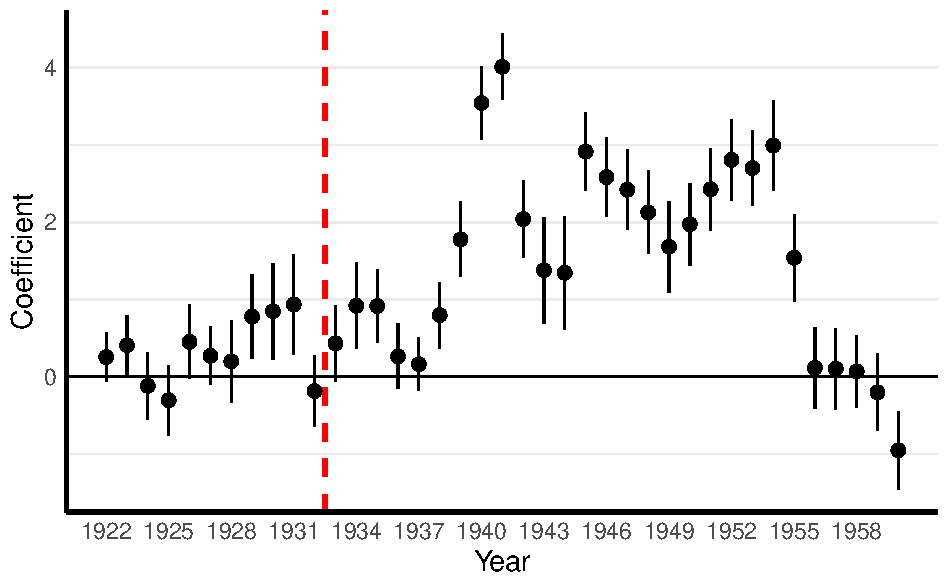
\includegraphics[width=\textwidth]{fmla_pred_full_imp_date_no_trends_geopol_cr2.pdf}
%\begin{minipage}{12\textwidth}
%\footnotesize
%\emph{Notes:} Ethnicity and date of arrest were imputed.  Full matrix adjustment was applied on ethnic group imputations. All 38 ethnic groups are included. There are no ethnicity-specific time trends. Standard errors are clustered on the level of ethnicity and are based on cluster robust estimator by \citet{pustejovsky_small-sample_2018}. Error bars show 95\% confidence intervals. 
%\end{minipage}
\label{fig:did_effets}
\end{figure}
\end{frame}


%\begin{frame}{Synthetic Control Method}  \begin{figure}[h] \centering
%\caption{Comparison plot}
%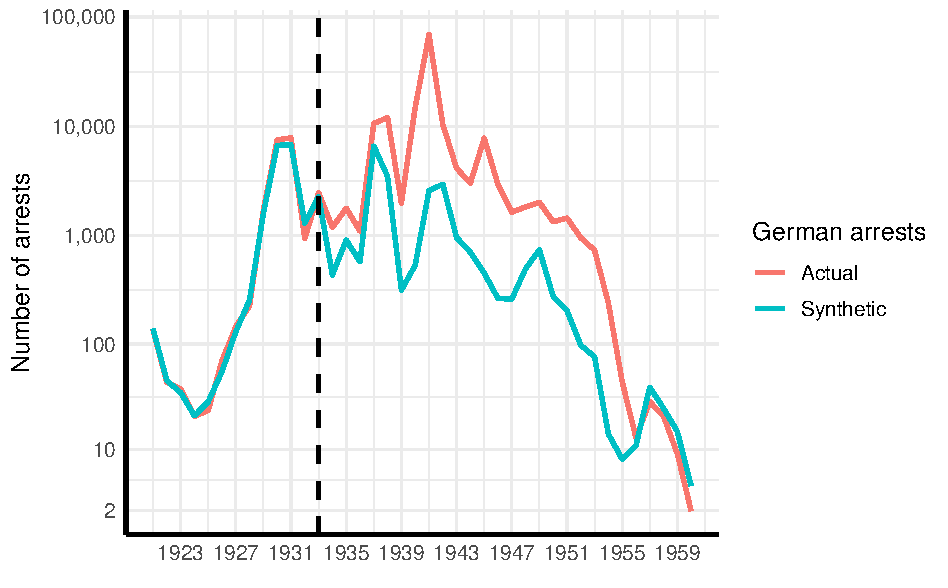
\includegraphics[width=1\textwidth]{comparison_plot_scaled.pdf}
%\begin{minipage}{0.92\textwidth}
%\includegraphics[width=\linewidth]{Gaus.pdf}
%\rule{\linewidth}{10em}
%\footnotesize
%\emph{Notes:} The values on y-axis are shown on $\log\left(1 + y\right)$ scale.  Ethnicity and date of arrest were imputed.  Full matrix adjustment was applied on ethnic group imputations. All 38 ethnic groups are included. 
%\end{minipage} 
%\label{fig:sc_comp_plot} \end{figure} \end{frame}




\begin{frame}{Synthetic Control Method}
 \begin{figure}[h]
\centering
%\caption{Comparison plot}
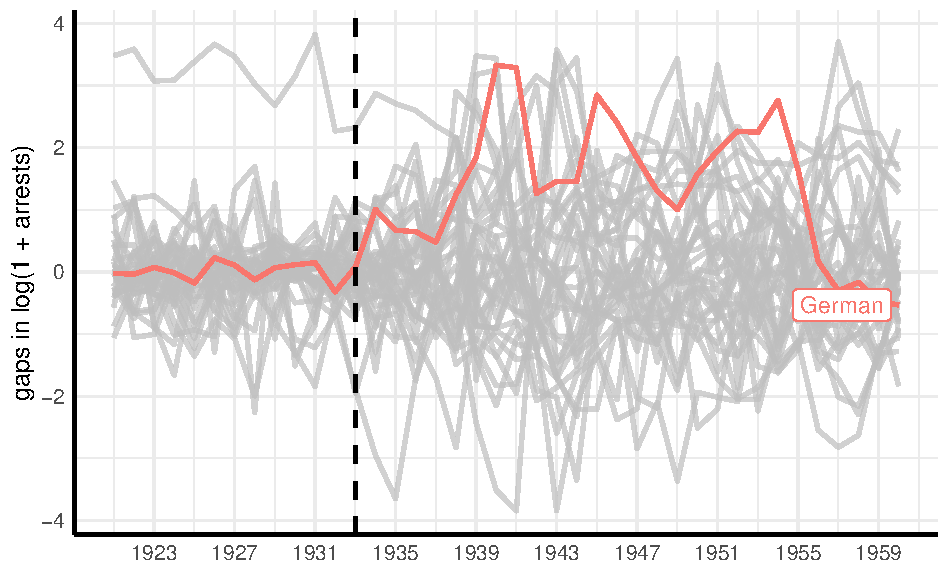
\includegraphics[width=1\textwidth]{placebo_highlight_all_imp_date.pdf}
\label{fig:sc_placebo_gaps_all}
\end{figure}
\end{frame}

%\begin{frame}{SC - MSPE Ratios} \begin{figure}[h] \centering 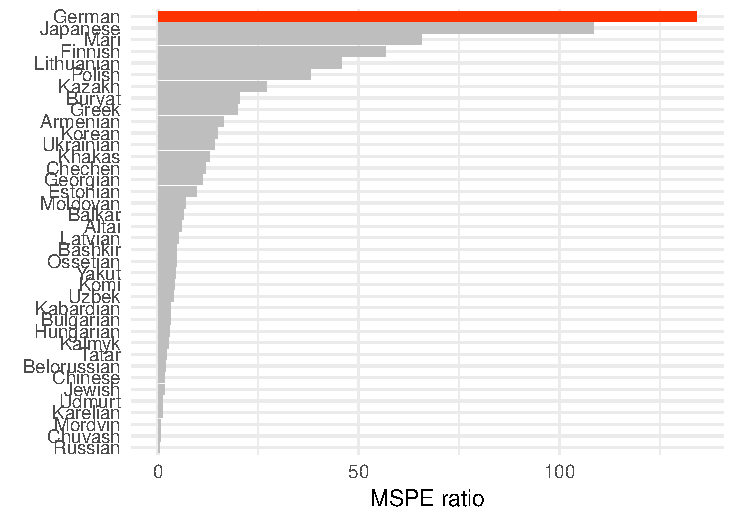
\includegraphics[width=1\textwidth]{mspe_ratios_imp_date.pdf} \label{fig:mspe_ratios_imp_date} \end{figure} \end{frame}



%\begin{frame}{SC - MSPE Ratios - Only 1933-1939 in Numerator}  \begin{figure}[h] \centering 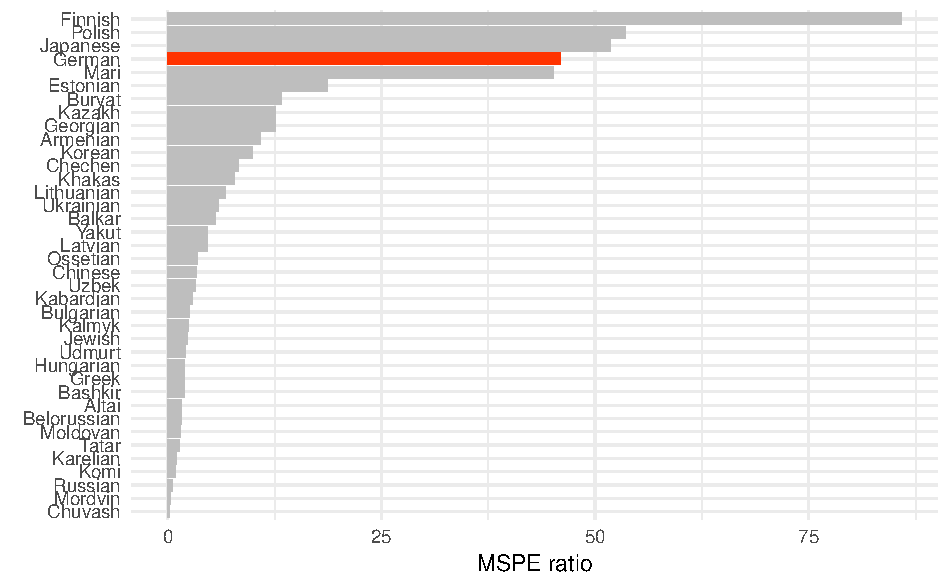
\includegraphics[width=1\textwidth]{mspe_ratios_imp_date_until_1939.pdf} \label{fig:mspe_ratios_imp_date_until_1939} \end{figure} \end{frame}

\begin{frame}[label=robustness_checks]{Difference-in-differences - Robustness Checks}
%\begin{itemize}
%    \item  Difference-in-differences
    \begin{itemize}
        \item Only ethnic groups without independent state \hyperlink{did_without_ind_state}{\beamergotobutton{here}}
        \item Only rehabilitated individuals \hyperlink{did_rehabs}{\beamergotobutton{here}}
        \item Only arrests from 250 km border frontier \hyperlink{did_border_area}{\beamergotobutton{here}}
        \item Only arrests outside 250 km border frontier \hyperlink{did_non_border_area}{\beamergotobutton{here}}
        \item Ethnicity-specific time trends  \hyperlink{did_time_trends}{\beamergotobutton{here}}
        \item Different ethnicity imputation adjustments (none, parsimonious, full matrix)   \hyperlink{did_pred_adj}{\beamergotobutton{here}}
        \item Stata standard errors  \hyperlink{did_stata_se}{\beamergotobutton{here}}
        \item Different base years 
        \begin{itemize}
            \item The whole pre-treatment period (1921-1932) omitted \hyperlink{did_from_1933}{\beamergotobutton{here}}
            \item Years 1921-1926 omitted \hyperlink{did_from_1927}{\beamergotobutton{here}}
        \end{itemize}

    \end{itemize}
%\end{itemize}
\end{frame}



\begin{frame}[label=sc_robustness_checks]{Synthetic Control - Robustness Checks}
%\begin{itemize}
%    \item  Difference-in-differences
 \begin{itemize}
    \item Mean of the outcome used as a predictor (instead of all pre-treatment outcomes) \hyperlink{sc_mean}{\beamergotobutton{here}}
        \item Only ethnic groups without independent state \hyperlink{sc_without_ind_state}{\beamergotobutton{here}}
        \item Only rehabilitated individuals \hyperlink{sc_rehabs}{\beamergotobutton{here}}
        \item Only arrests from 250 km border frontier \hyperlink{sc_border_area}{\beamergotobutton{here}}
        \item Only arrests outside 250 km border frontier \hyperlink{sc_non_border_area}{\beamergotobutton{here}}
       % \item Ethnicity-specific time trends  \hyperlink{did_time_trends}{\beamergotobutton{here}}
        %\item Different ethnicity imputation adjustments (none, parsimonious, full matrix)   \hyperlink{did_pred_adj}{\beamergotobutton{here}}
        %\item Stata standard errors  \hyperlink{did_stata_se}{\beamergotobutton{here}}
        %\item Different base years  \hyperlink{did_stata_se}{\beamergotobutton{here}}
    \end{itemize}
%\end{itemize}
\end{frame}


\section{Conclusion}

\begin{frame}{Conclusion}
\begin{itemize}
   % \item 
    \item Large and significant increase in repressions with war
    \item Strong persistence of the effect of war (nearly 10 years)
    \begin{itemize}
        \item This might suggest that strategic concerns are less important than desire for collective punishment 
    \end{itemize}
    \item Not limited to border frontiers (contrary to \citet{mcnamee_demographic_2019})
\end{itemize}

\end{frame}


{\setbeamercolor{palette primary}{fg=black, bg=white}
\begin{frame}[standout]
  Thank you for your attention.
\end{frame}
}

\appendix

\begin{frame}[allowframebreaks]{References}
\printbibliography
\end{frame}

\begin{frame}[label=add_content]{Additional Analyses}
\begin{itemize}
    \item Map of German population in the USSR \hyperlink{map_counts}{\beamergotobutton{here}}
    \item No imputation of date of arrest
    \hyperlink{did_no_date_imputation}{\beamergotobutton{DiD}} 
    \hyperlink{sc_no_date_imputation}{\beamergotobutton{SCM}} 
    \item Considering only western border areas 
    \begin{itemize}
        \item   Only arrests from western border areas 
        \hyperlink{did_border_area_west}{\beamergotobutton{DiD}} 
      \hyperlink{sc_border_area_west}{\beamergotobutton{SCM}} 
        \item Arrests from western border areas excluded
         \hyperlink{did_non_border_area_west}{\beamergotobutton{DiD}} 
      \hyperlink{sc_non_border_area_west}{\beamergotobutton{SCM}} 
        
    \end{itemize}
\end{itemize}
\end{frame}


\begin{frame}{Replication}
The R scripts and the LaTeX source codes of the thesis manuscript are available at:
  \begin{center}\url{https://github.com/martin-kosiik/Geopolitics-of-Repressions}\end{center}

The Beamer source code for this presentation itself are available at: 
\begin{center}\url{https://github.com/martin-kosiik/presentation-geopolitics-of-repressions}\end{center}
\end{frame}



\begin{frame}[label=ethnicity_imputation]{Ethnicity imputation}
\begin{itemize}
    \item Let  $\boldsymbol{x} = \left(x_1, x_2, x_3\right)$ be person's first, last, and patronymic names
    \item Assuming conditional independence, we can express probability that a person has ethnicity $E_k$ given his names as:
    \begin{equation*}
p(E_k \mid \mathbf{x}) = \frac{p(E_k) \ p(\mathbf{x} \mid E_k)}{p(\mathbf{x})}
\end{equation*}
    \item Naive Bayes classifier chooses ethnicity with the highest posterior probability as its prediction

\end{itemize}
\hyperlink{data}{\beamerreturnbutton{back}}
\end{frame}

\begin{frame}[label=arrest_date_imputation]{Imputing Missing Date of Arrest}
\begin{itemize}
    \item Date of arrest is missing for 1 650 912 observations 
    \begin{itemize}
        \item For 903 49 of them, date of trial is available - we use it for imputation
    \end{itemize}
    \item We model number of days between date of arrest and trial ($y$) in two-stages:
    \begin{enumerate}
        \item Logit to predict whether $y = 0$ (arrest and trial happening on the same day)
        \item  Log-linear regression on the subset of the data for which $y > 0$ 
    \end{enumerate}
    %\item The predicted (imputed) value is $\hat y_i = \hat I_i^y \cdot \hat y_i^{\text{pos}}$
\end{itemize}
\hyperlink{data}{\beamerreturnbutton{back}}
\end{frame}



\begin{frame}[label=did_without_ind_state]{DiD - Only Ethnicities without Independent State}
 \begin{figure}[h]
\centering
%\caption{Comparison plot}
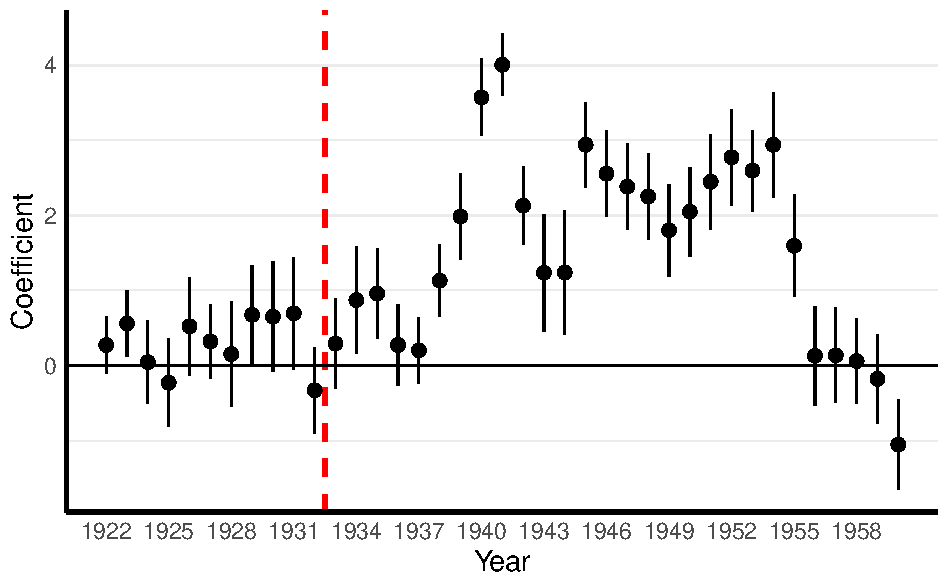
\includegraphics[width=1\textwidth]{pr_cr2_date_imp_full_years_no_trends_not_ind_country.pdf}
%\label{fig:sc_placebo_gaps_all}
\end{figure}

\hyperlink{robustness_checks}{\beamerreturnbutton{back}}
\end{frame}

\begin{frame}[label=did_rehabs]{DiD - Only Rehabilitated Individuals}
 \begin{figure}[h]
\centering
%\caption{Comparison plot}
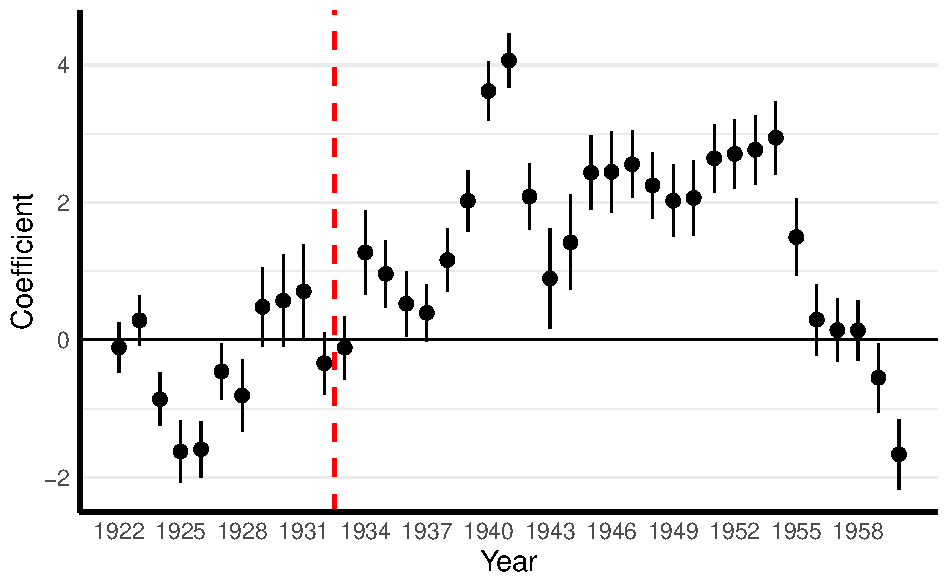
\includegraphics[width=1\textwidth]{fmla_pred_full_imp_date_no_trends_geopol_rehab_cr2.pdf}
%\label{fig:sc_placebo_gaps_all}
\end{figure}
\hyperlink{robustness_checks}{\beamerreturnbutton{back}}
\end{frame}

\begin{frame}[label=did_border_area]{DiD - Only arrests from Border Areas}
 \begin{figure}[h]
\centering
%\caption{Comparison plot}
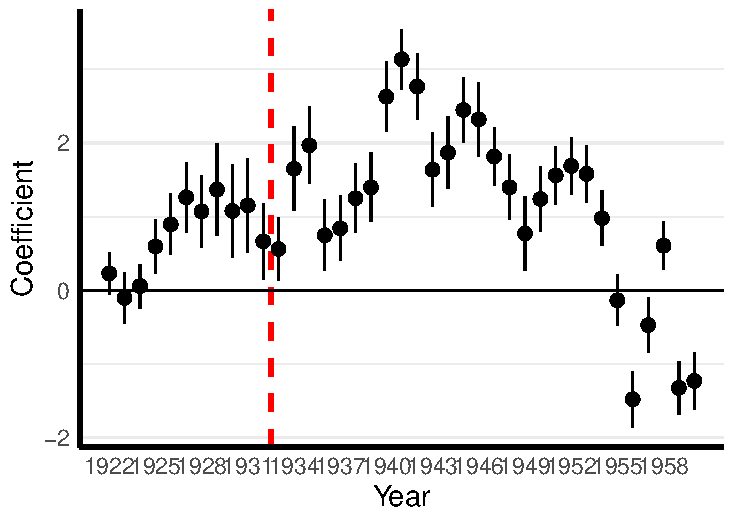
\includegraphics[width=1\textwidth]{point_range_robust_cr2_border_provinces.pdf}
%\label{fig:sc_placebo_gaps_all}
\end{figure}
\hyperlink{robustness_checks}{\beamerreturnbutton{back}}
\end{frame}


\begin{frame}[label=did_border_area_west]{DiD - Only arrests from Western Border Areas}
 \begin{figure}[h]
\centering
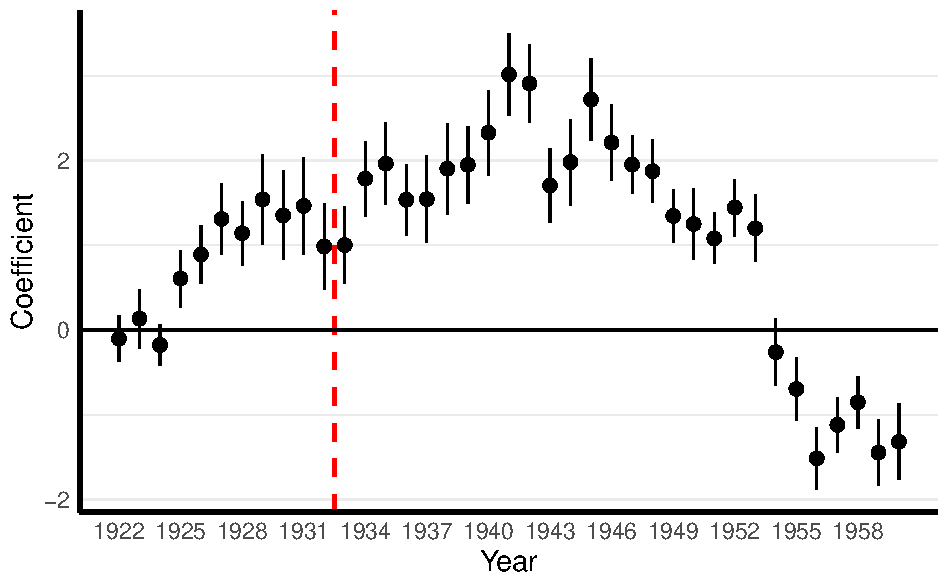
\includegraphics[width=1\textwidth]{point_range_robust_cr2_border_provinces_western.pdf}
%\label{fig:sc_placebo_gaps_all}
\end{figure}
\hyperlink{add_content}{\beamerreturnbutton{back}}
\end{frame}


\begin{frame}[label=did_non_border_area]{DiD - Arrests from Border Areas Excluded}
 \begin{figure}[h]
\centering
%\caption{Comparison plot}
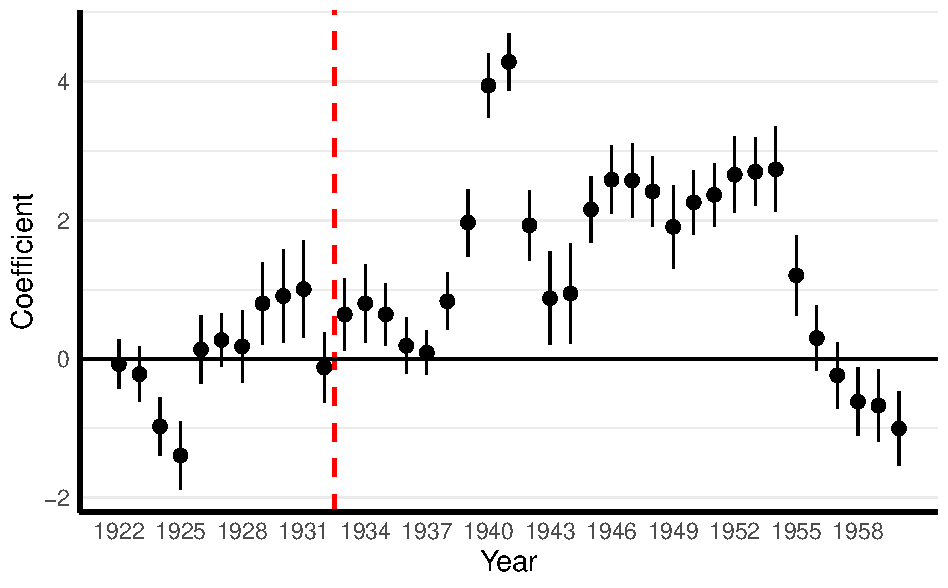
\includegraphics[width=1\textwidth]{point_range_robust_cr2_non_border_provinces.pdf}
%\label{fig:sc_placebo_gaps_all}
\end{figure}
\hyperlink{robustness_checks}{\beamerreturnbutton{back}}
\end{frame}


\begin{frame}[label=did_non_border_area_west]{DiD - Arrests from Western Border Areas Excluded}
 \begin{figure}[h]
\centering
%\caption{Comparison plot}
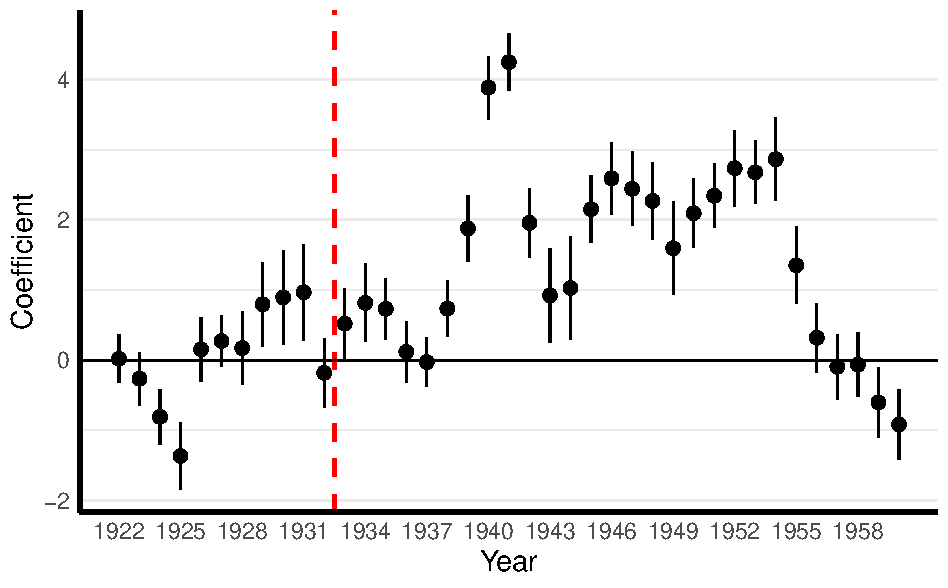
\includegraphics[width=1\textwidth]{point_range_robust_cr2_non_border_provinces_western.pdf}
%\label{fig:sc_placebo_gaps_all}
\end{figure}
\hyperlink{add_content}{\beamerreturnbutton{back}}
\end{frame}


\begin{frame}[label=did_time_trends]{DiD - Ethnicity-specific time trends}
 \begin{figure}[h]
\centering
%\caption{Comparison plot}
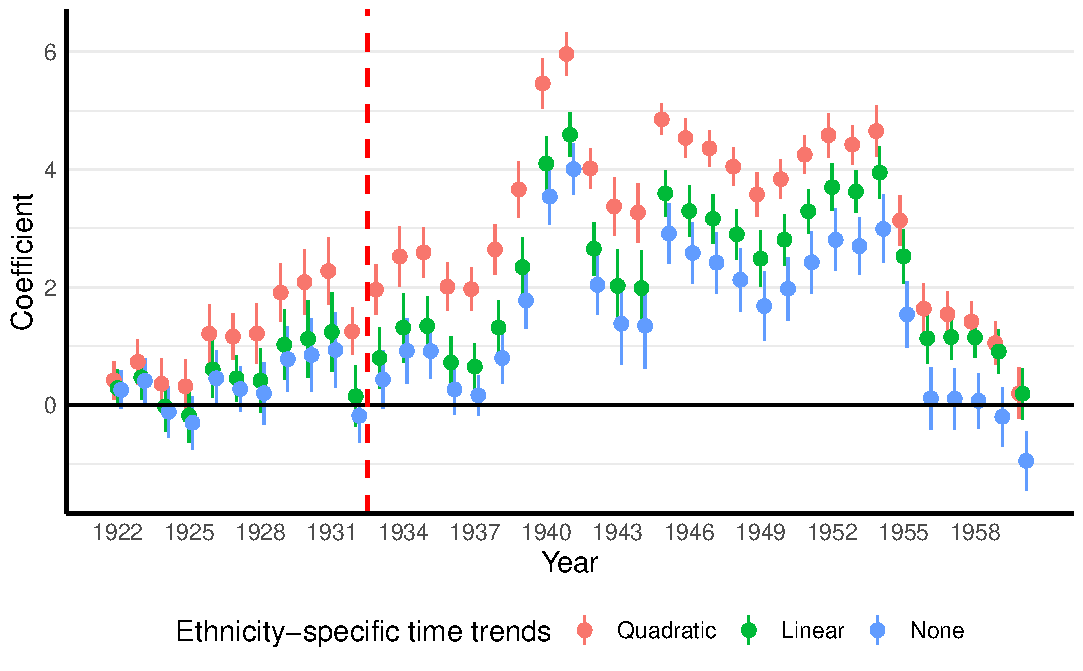
\includegraphics[width=1\textwidth]{trends_comp_pred_full_imp_date_cr2.pdf}
%\label{fig:sc_placebo_gaps_all}
\end{figure}
\hyperlink{robustness_checks}{\beamerreturnbutton{back}}
\end{frame}

\begin{frame}[label=did_pred_adj]{DiD - Different Ethnicity Imputation Adjustments}
 \begin{figure}[h]
\centering
%\caption{Comparison plot}
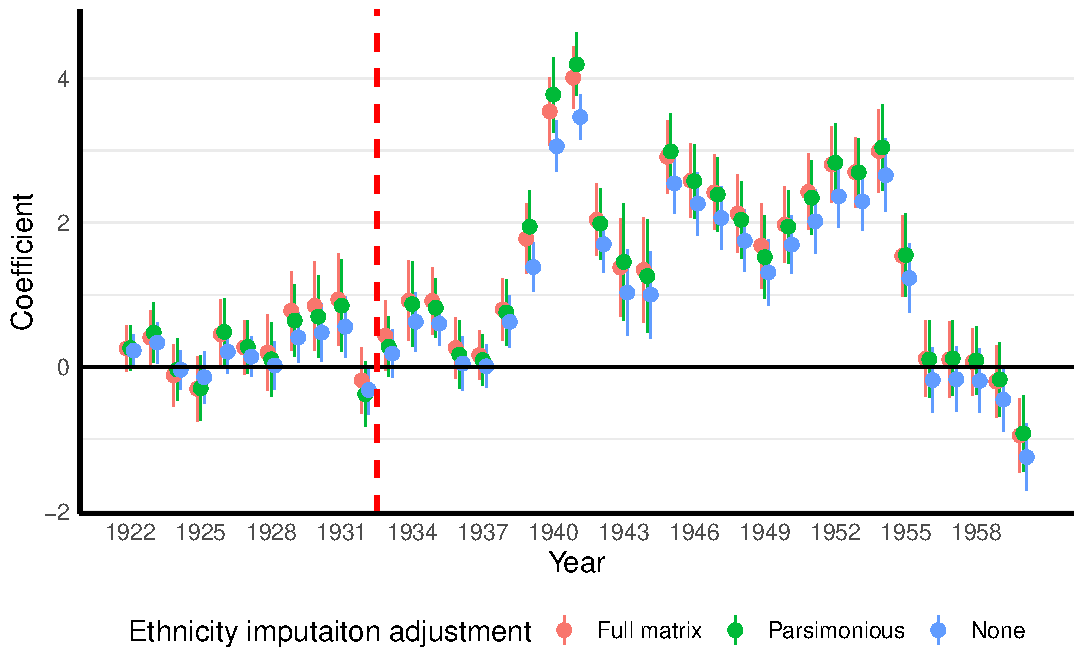
\includegraphics[width=1\textwidth]{pred_adj_comp_pred_full_imp_date_cr2.pdf}
%\label{fig:sc_placebo_gaps_all}
\end{figure}
\hyperlink{robustness_checks}{\beamerreturnbutton{back}}
\end{frame}


\begin{frame}[label=did_stata_se]{DiD - Stata Standard Errors}
 \begin{figure}[h]
\centering
%\caption{Comparison plot}
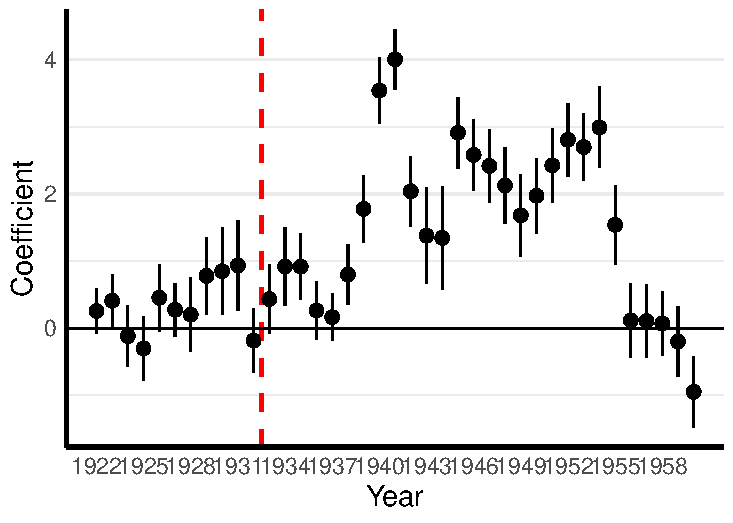
\includegraphics[width=1\textwidth]{fmla_pred_full_imp_date_no_trends_geopol_stata_SE.pdf}
%\label{fig:sc_placebo_gaps_all}
\end{figure}
\hyperlink{robustness_checks}{\beamerreturnbutton{back}}
\end{frame}

\begin{frame}[label=did_from_1927]{DiD - From 1927}
 \begin{figure}[h]
\centering
%\caption{Comparison plot}
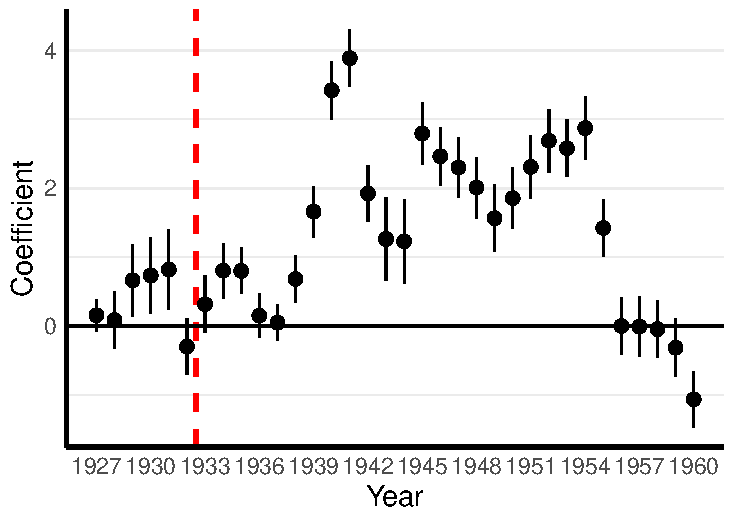
\includegraphics[width=1\textwidth]{pred_full_imp_date_no_trends_geopol_cr2_base_1927.pdf}
%\label{fig:sc_placebo_gaps_all}
\end{figure}
\hyperlink{robustness_checks}{\beamerreturnbutton{back}}
\end{frame}


\begin{frame}[label=did_from_1933]{DiD - From 1933}
 \begin{figure}[h]
\centering
%\caption{Comparison plot}
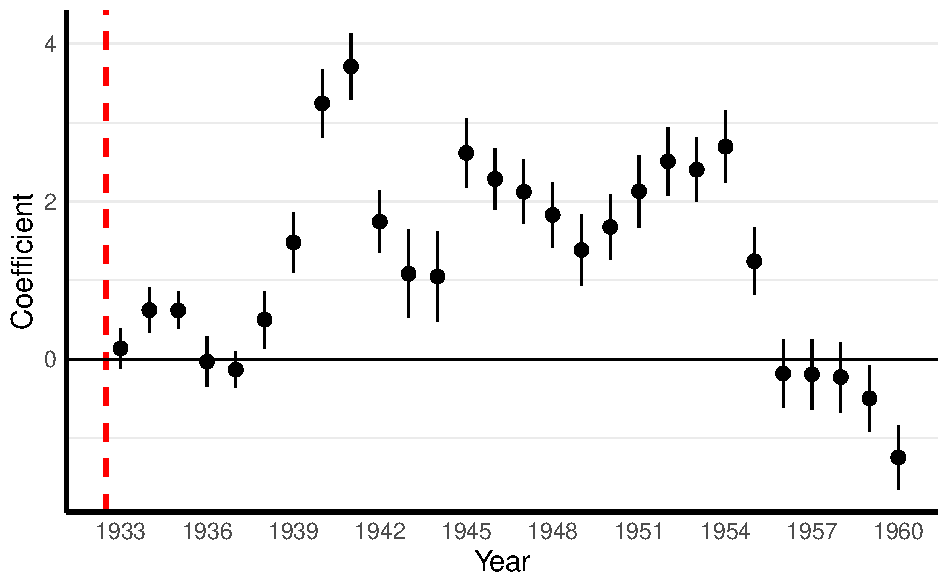
\includegraphics[width=1\textwidth]{pred_full_imp_date_no_trends_geopol_cr2_base_1933.pdf}
%\label{fig:sc_placebo_gaps_all}
\end{figure}
\hyperlink{robustness_checks}{\beamerreturnbutton{back}}
\end{frame}



\begin{frame}[label=sc_mean]{SCM - Mean of the Outcome as a Predictor}
 \begin{figure}[h]
\centering
%\caption{Comparison plot}
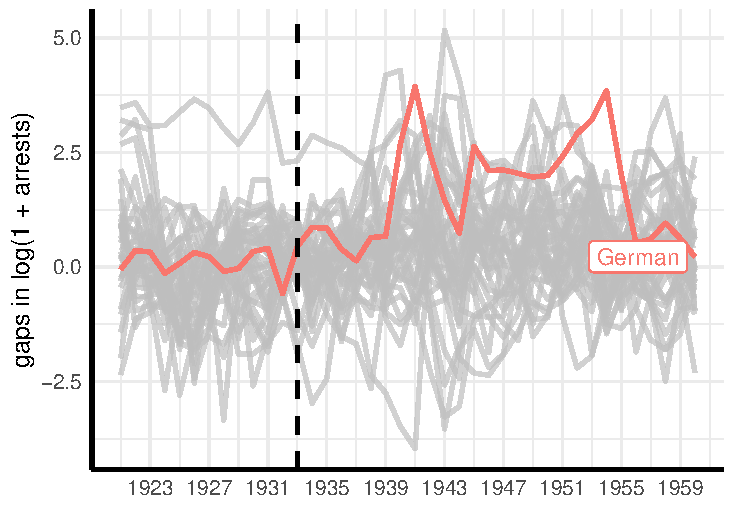
\includegraphics[width=1\textwidth]{placebo_highlight_all_imp_date_robustnes.pdf}
%\label{fig:sc_placebo_gaps_all}
\end{figure}
\hyperlink{sc_robustness_checks}{\beamerreturnbutton{back}}
\end{frame}

\begin{frame}[label=sc_without_ind_state]{SCM - Only Ethnicities without Independent State}
 \begin{figure}[h]
\centering
%\caption{Comparison plot}
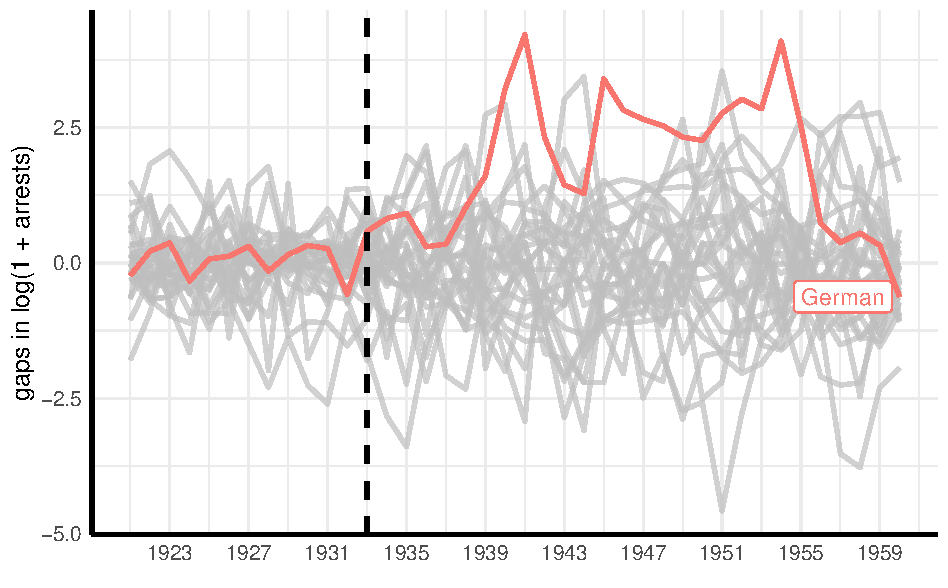
\includegraphics[width=1\textwidth]{placebo_highlight_all_ethnicities_without_ind_state.pdf}
\end{figure}
\hyperlink{sc_robustness_checks}{\beamerreturnbutton{back}}
\end{frame}

\begin{frame}[label=sc_rehabs]{SCM - Only Rehabilitated Individuals}
 \begin{figure}[h]
\centering
%\caption{Comparison plot}
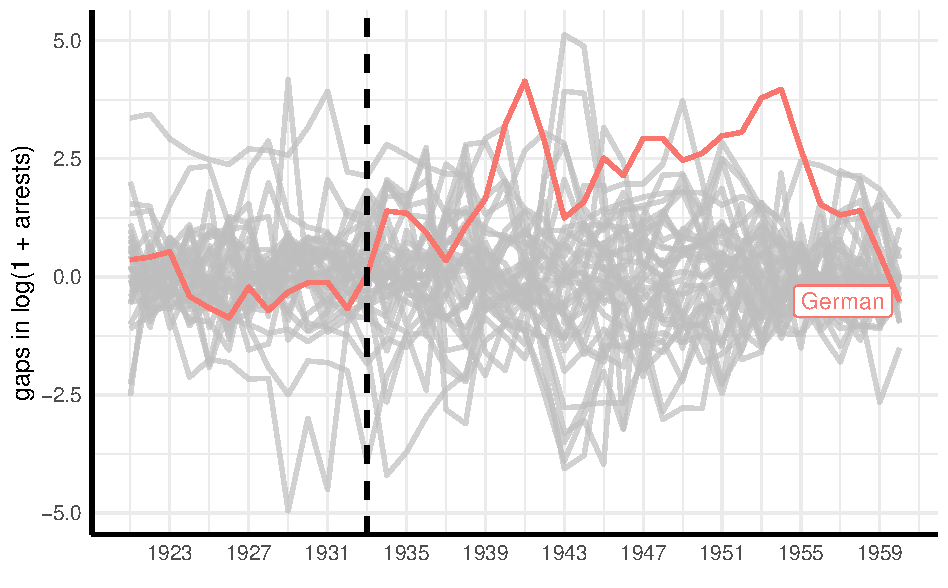
\includegraphics[width=1\textwidth]{placebo_highlight_all_rehabs.pdf}
\end{figure}
\hyperlink{sc_robustness_checks}{\beamerreturnbutton{back}}
\end{frame}

\begin{frame}[label=sc_border_area]{SCM - Only Arrests from Border Areas}
 \begin{figure}[h]
\centering
%\caption{Comparison plot}
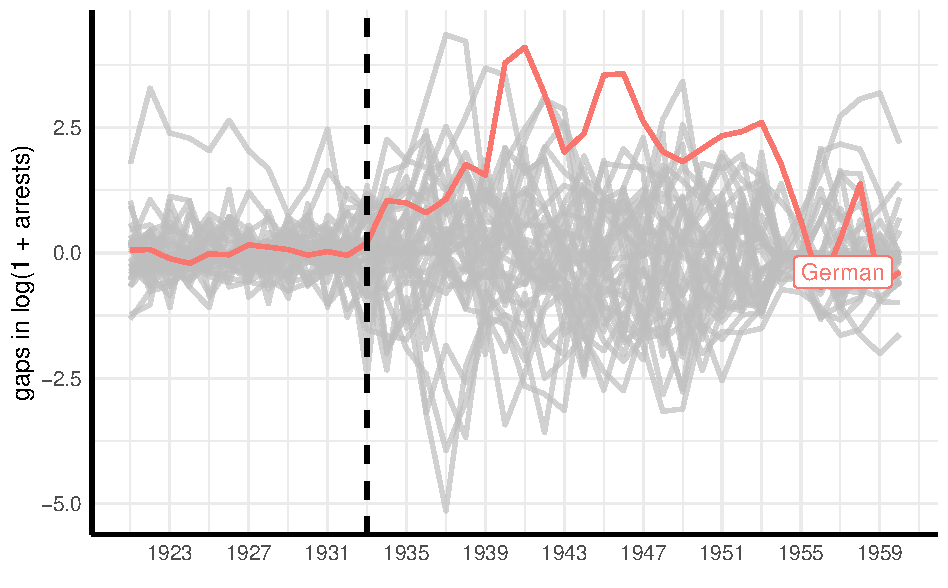
\includegraphics[width=1\textwidth]{placebo_highlight_all_border_provinces.pdf}
%\label{fig:sc_placebo_gaps_all}
\end{figure}
\hyperlink{sc_robustness_checks}{\beamerreturnbutton{back}}
\end{frame}

\begin{frame}[label=sc_border_area_west]{SCM - Only Arrests from Western Border Areas}
 \begin{figure}[h]
\centering
%\caption{Comparison plot}
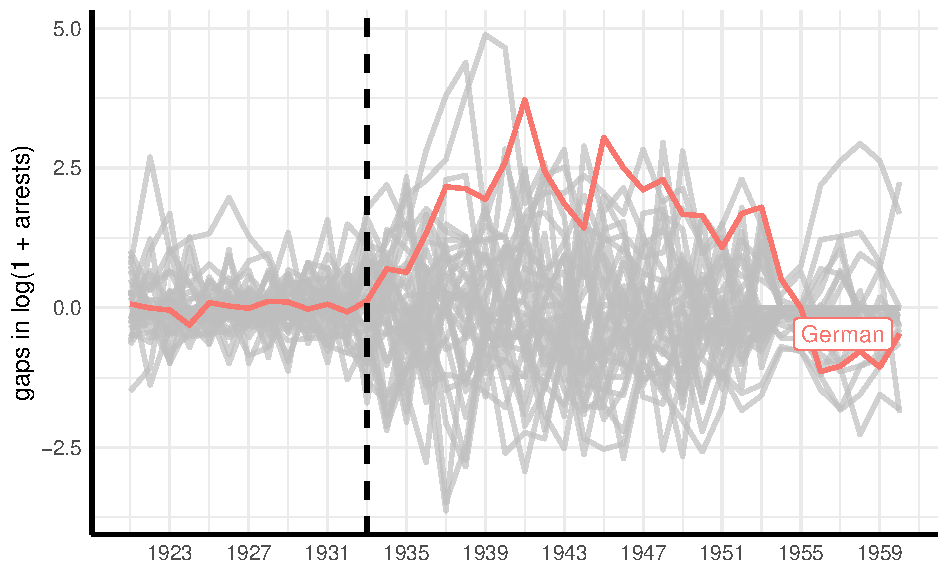
\includegraphics[width=1\textwidth]{placebo_highlight_all_border_provinces_western.pdf}
%\label{fig:sc_placebo_gaps_all}
\end{figure}
\hyperlink{add_content}{\beamerreturnbutton{back}}
\end{frame}

\begin{frame}[label=sc_non_border_area]{SCM - Arrests from Border Areas Excluded}
 \begin{figure}[h]
\centering
%\caption{Comparison plot}
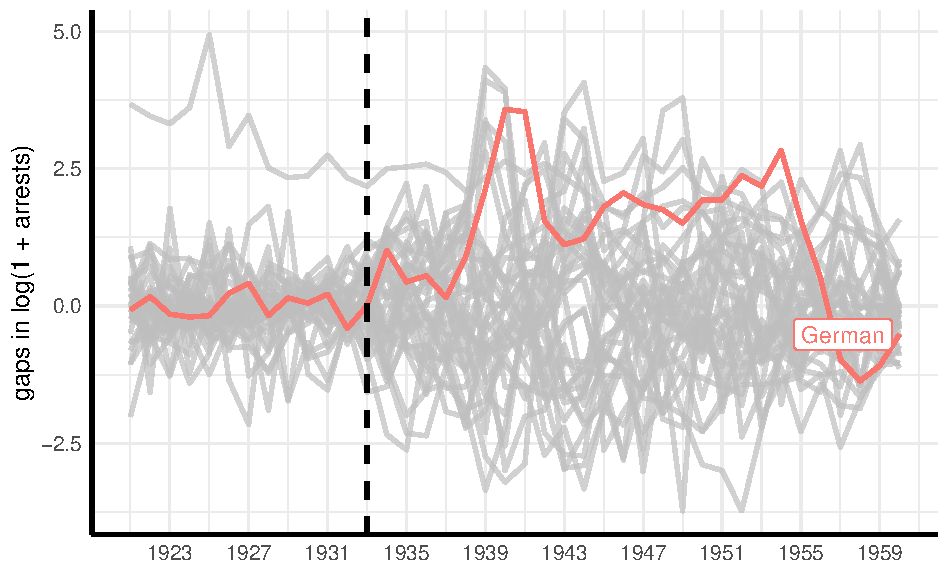
\includegraphics[width=1\textwidth]{placebo_highlight_all_non_border_provinces.pdf}
%\label{fig:sc_placebo_gaps_all}
\end{figure}
\hyperlink{sc_robustness_checks}{\beamerreturnbutton{back}}
\end{frame}


\begin{frame}[label=sc_non_border_area_west]{SCM - Arrests from Western Border Areas Excluded}
 \begin{figure}[h]
\centering
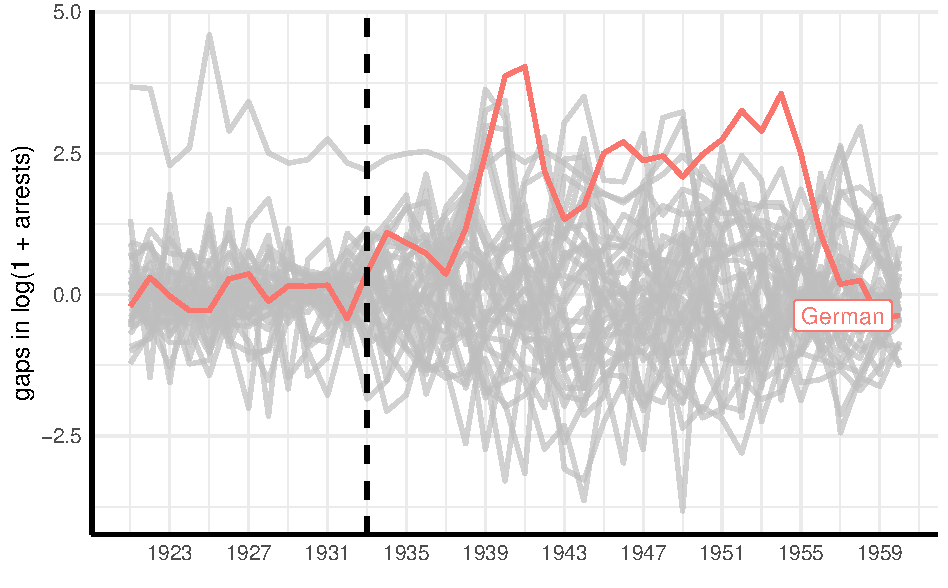
\includegraphics[width=1\textwidth]{placebo_highlight_all_non_border_provinces_western.pdf}
%\label{fig:sc_placebo_gaps_all}
\end{figure}
\hyperlink{add_content}{\beamerreturnbutton{back}}
\end{frame}


\begin{frame}[label=did_no_date_imputation]{DiD - No Imputations of Arrest Date}
 \begin{figure}[h]
\centering
%\caption{Comparison plot}
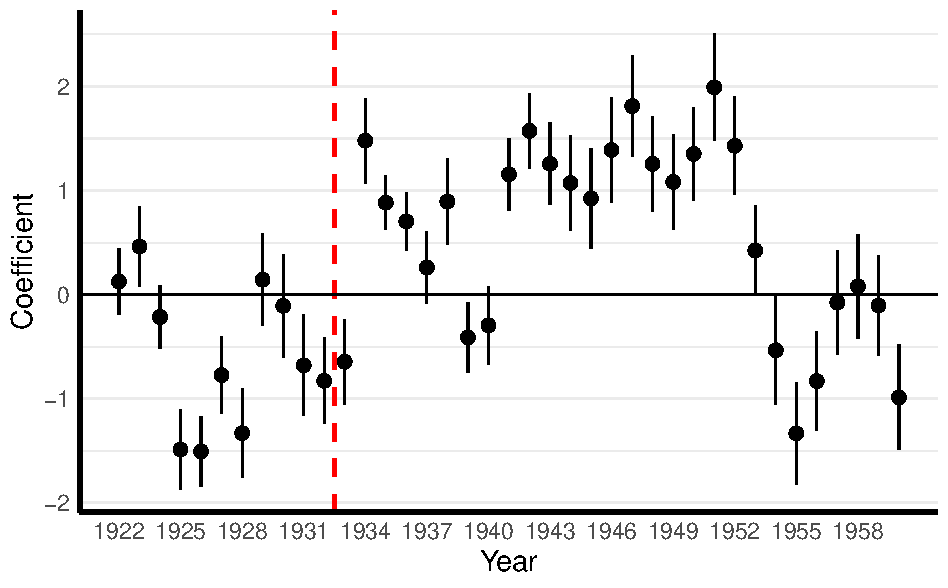
\includegraphics[width=1\textwidth]{pr_cr2_fmla_pred_full_no_trends_geopol.pdf}
%\label{fig:sc_placebo_gaps_all}
\end{figure}
\hyperlink{add_content}{\beamerreturnbutton{back}}
\end{frame}

\begin{frame}[label=sc_no_date_imputation]{SCM - No Imputations of Arrest Date}
 \begin{figure}[h]
\centering
%\caption{Comparison plot}
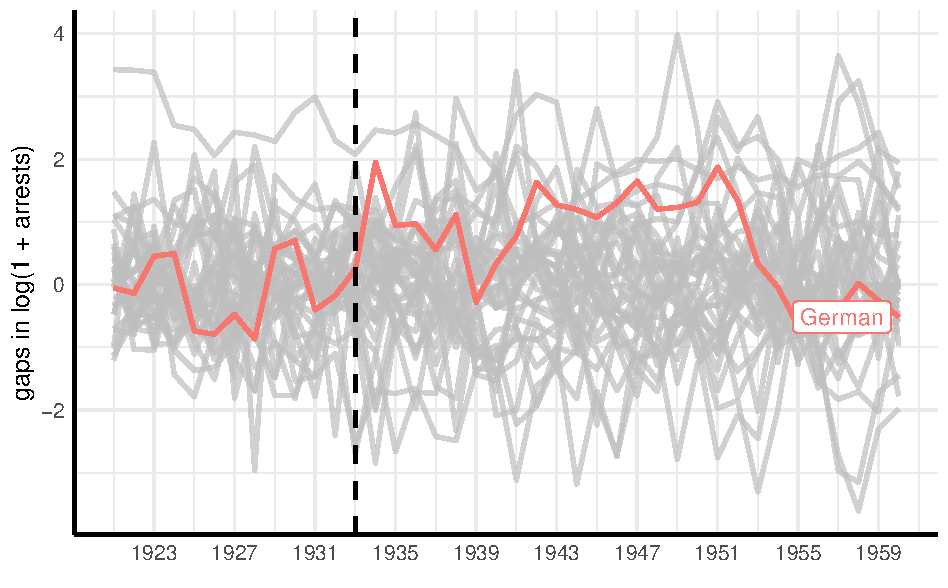
\includegraphics[width=1\textwidth]{placebo_highlight_all_no_date_imputation.pdf}
%\label{fig:sc_placebo_gaps_all}
\end{figure}
\hyperlink{add_content}{\beamerreturnbutton{back}}
\end{frame}


\begin{frame}[label=map_counts]{Map of German population in the USSR}
 \begin{figure}[h]
\centering
%\caption{Comparison plot}
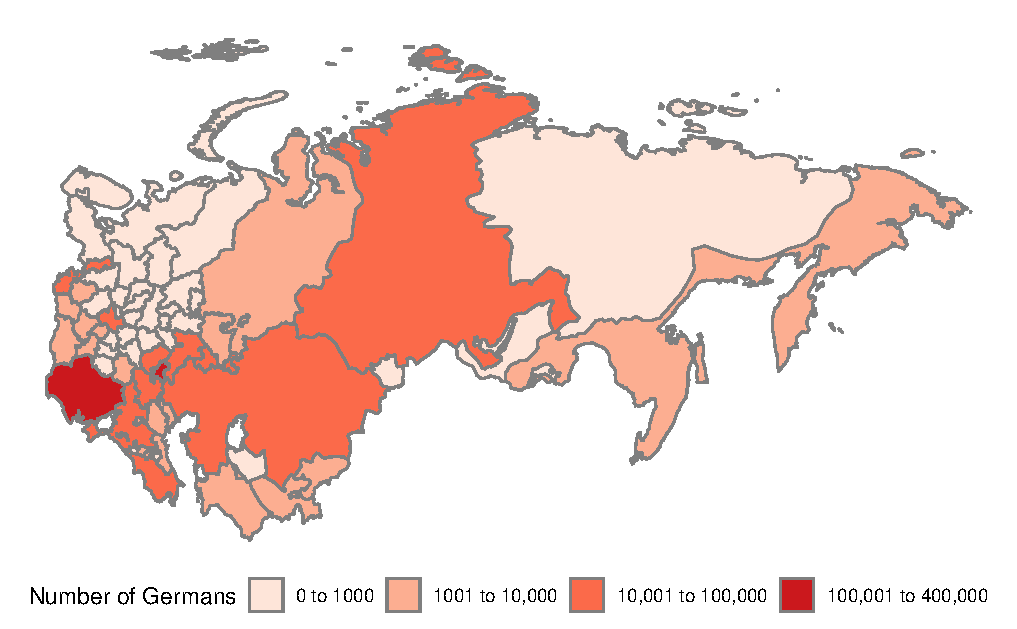
\includegraphics[width=1\textwidth]{map_number_of_germans_discrete.pdf}
%\label{fig:sc_placebo_gaps_all}
\end{figure}
\hyperlink{add_content}{\beamerreturnbutton{back}}
\end{frame}

\begin{frame}[label=map_share]{Map of German population in the USSR}
 \begin{figure}[h]
\centering
%\caption{Comparison plot}
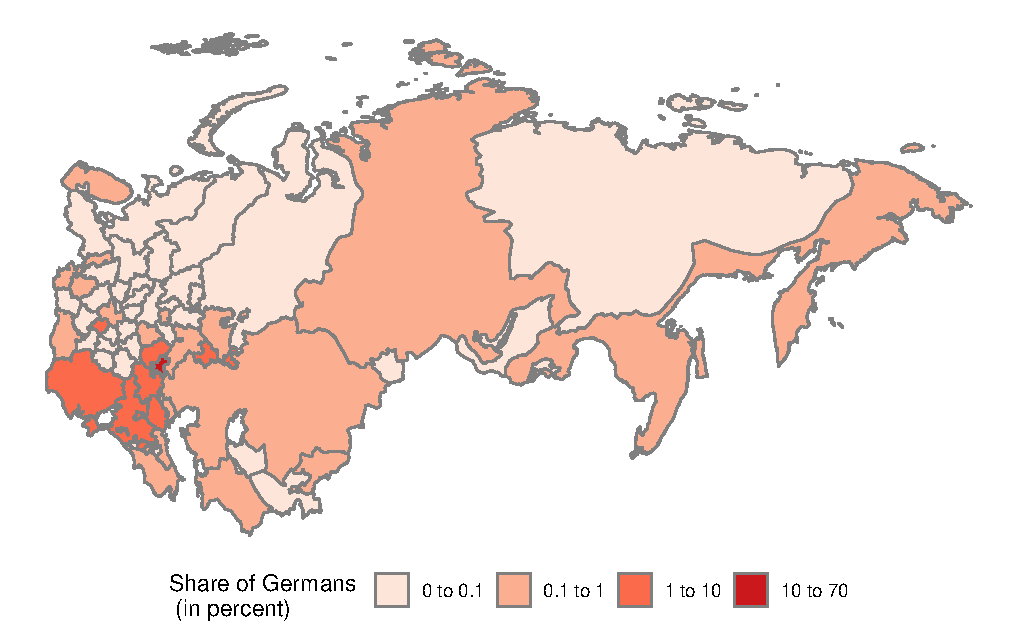
\includegraphics[width=1\textwidth]{map_share_of_germans_discrete.pdf}
%\label{fig:sc_placebo_gaps_all}
\end{figure}
\hyperlink{add_content}{\beamerreturnbutton{back}}
\end{frame}

\end{document}
